\chapter {KAJIAN PUSTAKA DAN DASAR TEORI}

Bab ini berisi pembahasan tentang dasar teori dan kajian pustaka yang digunakan sebagai teori pendukung penelitian ini. Terlebih dahulu akan dijelaskan mengenai kasus pencarian Ulam. Kemudian dilanjutkan dengan beberapa solusi pencarian Ulam yang sudah ada maupun teori pendukung solusi pencarian Ulam non-interaktif yaitu teori pengkodean dan kode biner.

\section{Kasus-kasus pencarian Ulam di online judge}

Pada online judge SPOJ, ada lima variasi soal yang diajukan seperti pada Tabel \ref{tab:kasus_spoj}. Jenis soal classical adalah jenis soal yang jawaban yang diajukan hanya dapat bernilai benar atau salah, sedangkan jenis soal challenge membolehkan jawaban yang diajukan adalah yang paling buruk ataupun yang paling baik. Pada soal challenge, terdapat nilai skor dari jawaban yang diajukan.

Soal GUESSN1 dan GUESSN3 adalah pencarian Ulam dengan jumlah maksimal kebohongan satu dan tipe query interaktif. Soal jenis ini dapat diselesaikan dengan menentukan query dengan pembobotan Berlekamp $w_j (a,b)=a(j+1)+b$ di mana j adalah jumlah query tersisa, $a$ dan $b$ berturut adalah \textit{truth}-set dan \textit{lie}-set \cite{Pelc1987}.

\begin{table}[h!]
\caption{Daftar kasus pencarian Ulam di SPOJ}
\label{tab:kasus_spoj}
\begin{center}
\begin{tabular} {|l|l|l|l|l|l|}
\hline
Kode & Jumlah bohong & Jenis query & Tipe query & Jenis soal & Kesulitan \\
\hline
GUESSN1 & 1 & Subset & Interaktif & challenge & Mudah \\
\hline
GUESSN2 & 2-16 & Subset & Interaktif & challenge & Susah  \\
\hline
GUESSN3 & 1 & Range & Interaktif & classical & Menengah \\
\hline
GUESSN4 & 1 & Subset & Non-interaktif & challenge & Menengah \\
\hline
GUESSN5 & 2-16 & Subset & Non-interaktif & challenge & Sangat susah \\
\hline
\end{tabular}
\end{center}
\end{table}


\section{Formulasi permasalahan}

Bentuk permasalahan Ulam yang dibahas pada paper ini diangkat dari online judge SPOJ oleh Micha\l{} Miodek \cite{guessn5}. Penjawab menentukan sebuah bilangan $x$ pada rentang $S_M=\{0,\ldots,M-1\}$. Anda sebagai penanya harus mencari nilai $x$ dengan memberikan maksimal $n$ query khusus apakah "$x \in Q$?", lalu penjawab menjawab 'ya' atau 'tidak' pada setiap query yang ditanyakan. Permasalahan utama adalah penjawab dapat berbohong sampai $e$ kali. Selain itu, penjawab hanya boleh menjawab query penanya setelah penanya selesai menanyakan semua query-nya. Tujuan dari Ulam adalah mencari jumlah query minimal untuk dapat menentukan nilai $x$.

Bentuk dari query adalah string $s_1s_2s_3\ldots s_n$ di mana $s_i$ bernilai $0$ atau $1$. Jawaban dari penjawab adalah "Ya" jika $s_x=1$ atau "Tidak" jika $s_x=0$ dengan asumsi penjawab menjawab jujur.

Tugas sesungguhnya dari permasalahan ini adalah bukan untuk mencari nilai $x$, tapi hanya menyiapkan query yang dapat memeungkinkan untuk mendapatkan nilai $x$ dari semua kemungkinan jawaban dari penjawab. Penjawab tidak akan menjawab query yang diberikan penanya. Jika penjawab menemukan ada suatu set jawaban yang menyebabkan ada lebih dari satu kemungkinan nilai $x$, maka pengujian dianggap gagal.

\begin{figure}
\centering
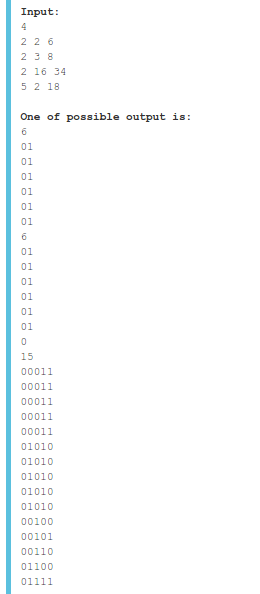
\includegraphics[scale=0.43]{../img/example.png}
\caption{Contoh kasus uji pada GUESSN5}
\label{fig:guessn5_test_case}
\end{figure}

Gambar \ref{fig:guessn5_test_case} adalah contoh empat uji kasus dari permasalahan SPOJ GUESSN5. Pada uji kasus yang pertama hanya terdapat dua angka. Jika penjawab tidak berbohong, penjawab dapat menjawab pilihan

\begin{center}
\begin{BVerbatim}
111111   000000.
\end{BVerbatim}
\end{center}

\noindent
Jika penjawab berbohong satu kali, penjawab dapat menjawab

% \begin{align*}
\begin{center}
\begin{BVerbatim}
111110   111101   111011
110111   101111   011111
000001   000010   000100
001000   010000   100000.
\end{BVerbatim}
\end{center}
% \end{align*}

\noindent
Jika penjawab berbohong dua kali, penjawab dapat menjawab

\begin{center}
\begin{BVerbatim}
000011   000101   000110
001001   001010   001100
010001   010010   010100
011000   100001   100010
100100   101000   110000
001111   010111   011011
011101   011110   100111
101011   101101   101110
110011   110101   110110
111001   111010   111100.
\end{BVerbatim}
\end{center}

\noindent
Penanya memenangkan permainan karena kemungkinan jawaban selain tersebut di atas membuat penjawab akan berbohong tiga kali.

Pada uji kasus yang kedua penjawab mencoba memberikan solusi namun jawabannya salah. Penanya dapat menjawab \texttt{111000} yaitu jawaban yang valid karena jumlah bohong tiga kali untuk kedua kemungkinan angka. Pada kasus ini penanya kalah karena penanya membutuhkan query tambahan.

Pada uji kasus yang ketiga penanya tidak memberikan solusi.

Pada uji kasus yang keempat penanya memberikan query yang lebih sedikit dari jumlah query maksimal yang diperbolehkan. Dari semua kemungkinan jawaban penjawab, pasti hanya ada satu jawaban nilai $x$, jadi penanya memenangkan permainan.


\section{Solusi pada permasalahan Ulam secara umum}

Pada permasalahan Ulam, penjawab menentukan sebuah angka $x$ di mana $x \in S_n$, lalu penanya akan menanyakan query untuk membantu mencari nilai $x$. Pada kenyataannya, penjawab tidak benar-benar memilih sebuah angka $x$, namun mempersiapkan $n$ angka dengan state keboongan dari setiap angka \cite{Pelc1987}. State kebohongan setiap angka dapat digambarkan dengan bipartite graph kanal untuk status kebohongan dari setiap bilangan $S_n$ \cite{Ahlswede2008}. Setiap kanal $C_i \subseteq S_n$ pada $C=\{C_0,C_1,\ldots,C_e\}$ adalah kanal berbentuk vektor yang berisi elemen dari $S_n$ dengan status jumlah kebohongan $i$ \cite{Ellis2005}.

Setiap query $Q=\{q_1,q_2,\ldots\} \mid q_i \in S_n$, dengan jawaban penjawab adalah "ya" maka set angka yang dianggap benar pada query tersebut adalah $Q_t=\{t_1,t_2,\ldots\} \mid t_i = q_i$ sedangkan jika jawaban penjawab adalah "tidak" maka set angka yang dianggap benar pada query tersebut adalah $Q_t=S_n-Q$. Semua angka yang dianggap salah yaitu pada $S_n-Q_t=\{t_1,t_2,\ldots\}$ akan dipindahkan ke state kanal setelahnya. Jika $t_i$ berasal dari $C_e$, maka $t_i$ akan dikeluarkan dari kanal, sehingga nilai $x$ pasti bukan $t_i$ karena melampaui jumlah bohong maksimal.

Kanal pada setiap state query dan jawaban query memiliki bobot, yaitu berapa kesempatan setiap nilai angka pada setiap kanal untuk berbohong, sampai akhirnya tereliminasi karena melampaui jumlah bohong maksimal. Setiap state dapat dinotasikan pada Persamaan \ref{eq:berlekamp}, di mana $wb$ adalah fungsi Berlekamp, $C$ adalah vektor kanal state, $c_i$ adalah jumlah elemen pada $C_i$, $k$ adalah jumlah query tersisa, dan $e$ adalah jumlah bohong maksimal. Notasi kombinatorik pada Persamaan \ref{eq:combinatoric} yaitu $q$ kombinasi $i$.

\begin{equation} \label{eq:berlekamp}
wb(C,k) = \sum^{e}_{i=0} c_i \binom{k}{\leq e-i}
\end{equation}

\begin{equation} \label{eq:combinatoric}
\binom{k}{\leq e} = \sum^{e}_{i=0} \binom{q}{i}
\end{equation}

Karakter dari state $C$  yang dapat dinotasikan sebagai $ch(C)$ yang ditunjukkan pada Persamaan \ref{eq:character} adalah jumlah pertanyaan minimal untuk dapat memenangkan permainan pada state $C$ \cite{Deppe2004}. Oleh karena itu penanya memiliki kemungkinan untuk memenangkan permainan jika $wb(C,k) \geq 2^k$ \cite{Ellis2005}.

\begin{equation} \label{eq:character}
ch(C) = \min\{k \mid wb(C,k) \leq 2^k\}
\end{equation}

Berdasarkan teori konservasi Berlekamp \cite{Deppe2004} $wb(C,k) = wb_y(C,k) + wb_n(C,k)$ yaitu bobot pada state $k$ sama dengan jumlah bobot pada state $k-1$ dengan jawaban penjawab "ya" dan "tidak". Oleh karena itu yang harus dilakukan adalah mempersiapkan query agar selisih bobot jawaban "ya" dan "tidak" sekecil mungkin untuk meminimalkan bobot.

Untuk mengetahui sebuah query memiliki selisih bobot jawaban "ya" dan "tidak" sekecil mungkin maka dibuatlah sebuah rumus seperti pada Persamaan \ref{eq:deltaj} di mana $j$ adalah state sisa pertanyaan, $Y$ dan $N$ adalah hasil $C$ ketika jawaban "ya" dan "tidak". Jika nilai $\Delta_j(C,Q) = 0$ maka dapat dikatakan bahwa query $a$ adalah sempurna pada state $j$. Namun karena penanya tidak dapat selalu membuat pertanyaan yang sempurna, maka akan dicari pertanyaan yang dapat menghasilkan $\Delta_j(C,Q)$ mendekati $0$.

\begin{equation}
\label{eq:deltaj}
\Delta_j(C,Q) = wb(Y(C,Q),j) - wb(N(C,Q),j)
\end{equation}


\section{Repetisi kode biner}

Ide pertama yang mungkin untuk menyelesaikan permasalahan ini adalah dengan mempersiapkan pencarian biner \cite{VanLint2016}. Query awal pencarian biner berjumlah $q_b=\log_2(M)$, agar setiap kemungkinan jawaban dari penjawab dapat mewakili semua kemungkinan nilai $x$. Lalu setiap query akan diulang sebanyak $q_e=2e+1$ kali agar penjawab pasti menjawab dengan jujur, karena $e$ query untuk jawaban bohong, ditambah dengan $e$ query untuk mengeliminasi jawaban bohong, ditambah dengan satu query jawaban pasti jujur karena kesempatan penjawab untuk berbohong sudah habis. Total jumlah query $q=q_b \times q_e$.

\begin{table}[h!]
\caption{Contoh pencarian biner pada $M=8$}
\label{tab:binary_8}
\begin{center}
\begin{tabular}{|l|c|c|c|c|c|c|c|c|}
\hline
$x$  & 1 & 2 & 3 & 4 & 5 & 6 & 7 & 8 \\
\hline
$Q_1$ & 0 & 0 & 0 & 0 & 1 & 1 & 1 & 1 \\
\hline
$Q_2$ & 0 & 0 & 1 & 1 & 0 & 0 & 1 & 1 \\
\hline
$Q_3$ & 0 & 1 & 0 & 1 & 0 & 1 & 0 & 1 \\
\hline
Jawaban & NNN & NNY & NYN & NYY & YNN & YNY & YYN & YYY \\
\hline
\end{tabular}
\end{center}
\end{table}

Misalnya jika $M=8$, $e=2$, maka jumlah $q_b$ untuk pencarian biner adalah \texttt{00001111}, \texttt{00110011} dan \texttt{01010101} seperti pada Tabel \ref{tab:binary_8}. Dari tiga query, tersebut, semua jawaban penjawab mulai dari "NNN" sampai "YYY" dapat mewakili semua nilai $x$ dalam $S_M={1,2,...,8}$ sehingga nilai $q_b=3$. Lalu masing-masing query diulang sebanyak $q_e=2e+1=5$ kali. Maka total dari $q=q_b \times q_e=9$.


\section{Teori pengkodean}

Tujuan utama dari teori pengkodean (\textit{coding theory}) adalah bagaimana mengirimkan pesan pada kanal yang mengandung derau (\textit{noisy channel}) \cite{VanLint2016}. Misal jika ada delapan macam kata pesan yang akan dikirim, maka kita merepresentasikan pesan tersebut menjadi bitstring biner dengan panjang 3. Namun jika pesan tersebut dikirm langsung melewati kanal yang mengandung derau, bisa jadi misalkan ada 1 bit akan tertukar, misal \texttt{001} menjadi \texttt{011}. Jika terjadi seperti itu, maka sebuah kata dapat tertukar menjadi kata yang lain.

Kita tahu bahwa jika kode biner sepanjang $n$ digunakan untuk membuat $2^n$ bitstring tidak dapat mendeteksi eror. Ide yang paling mungkin adalah pengirim dan penerima menyetujui sebuah metode enkripsi bitstring menjadi bitstring yang lebih panjang dan dapat mendeteksi maksimal sebanyak $e$ error menggunakan kode linear.

Kode linear adalah kode yang paling banyak dipelajari karena struktur aljabar yang mudah dipelajari dibandingkan kode non-linear \cite{Huffman}. Bidang kode linear dapat dinotasikan sebagai $\mathbb{F}_q^n$, yaitu kode memiliki $q$ jenis elemen dan memiliki panjang $n$. Bentuk kode biner adalah $\mathbb{F}_2^n$, memiliki struktur aljabar penjumlahan dan perkalian pada Gambar \ref{fig:algebra}.

\begin{figure}
\centering
\begin{align*}
0 + 0 &= 0 & 0 \cdot 0 &= 0 \\
0 + 1 &= 1 & 0 \cdot 1 &= 0 \\
1 + 0 &= 1 & 1 \cdot 0 &= 0 \\
1 + 1 &= 0 & 1 \cdot 1 &= 1
\end{align*}
\caption{Operasi linear pada $\mathbb{F}_2$}
\label{fig:algebra}
\end{figure}

\begin{equation} \label{eq:dh}
d_H(\vec{x},\vec{y}) = |\{i \in {1,\ldots,n} \mid x_i \neq y_i\}|
\end{equation}

Jarak Hamming dari bitstring $\vec{x}$ dan $\vec{y}$ dengan panjang $n$ didefinisikan dengan Persamaan \ref{eq:dh} \cite{Cicalese2000}. Sebagai contohnya $d_H(\texttt{0000},\texttt{1111})= 4$ dan $d_H(\texttt{00110},\texttt{00101})= 2$. $d_H(\vec{x},\vec{y})$ juga dapat dikatakan jumlah minimal untuk mentransformasi dari $\vec{x}$ ke $\vec{y}$. Contoh $\vec{x}=\texttt{00110}$ dan $\vec{y}=\texttt{00101}$ memiliki perbedaan pada 2 bit terakhir dengan jarak Hamming 2, dapat dikatakan $\vec{x}+\texttt{00011} = \vec{y}$.

\begin{equation} \label{eq:wt}
wt(\vec{x}) = |\{i \in {1,\ldots,n} \mid x_i \neq 0\}|
\end{equation}

Bobot dari bitstring $\vec{x}$ didefinisikan dengan $wt(\vec{x})$, yaitu jumlah digit pada $\vec{x}$ yang bukan \texttt{0} seperti pada Persamaan \ref{eq:wt}. Sebagai contohnya, $wt(\texttt{00101}) = 2$ dan $wt(\texttt{11111}) = 5$. Jika dihubungkan dengan jarak Hamming, jika $\vec{x}+\vec{e} = \vec{y}$ maka $d_H(\vec{x},\vec{y}) = wt(\vec{x}+\vec{y})$.

Terdapat sebuah sifat pada jarak Hamming yang bernama segitiga pertidaksamaan (\textit{triangle inequality}) \cite{VanLint2016}.
\begin{equation} \label{eq:dh_unequal}
d_H(\vec{x},\vec{y}) \le d_H(\vec{x},\vec{z}) + d_H(\vec{y},\vec{z})
\end{equation}
Dari Persamaan \ref{eq:dh_unequal}, misalkan $\vec{z}$ adalah $\vec{0}$ yaitu string biner yang berisi semua \texttt{0}, maka didapatkan Persamaan \ref{eq:wt_unequal}.
\begin{equation} \label{eq:wt_unequal}
wt(\vec{x}+\vec{y}) \le wt(\vec{x}) + wt(\vec{y})
\end{equation}


\section{Kode biner}

Kode biner (\textit{binary code}) adalah sejumlah $M$ bitstring biner dengan panjang masing-masing bitstring adalah $n$ dan jarak Hamming pada masing masing bitstring adalah $d$. Mari kita ambil contoh $M=8$, $n=6$, dan $d=3$ pada Gambar \ref{fig:binarycode683}. Parameter pada kode ini adalah $(6,8,3)_2$, yaitu kode biner yang ditunjukkan pada angka 2, panjang bitstring 6, berisi 8 bitstring, dengan jarak Hamming minimal 3. Bitstring pada kode biner selanjutnya disebut kata kode (\textit{codeword}).

\begin{figure}
\centering
\begin{BVerbatim}
000000  100110
001011  101101
010101  110011
011110  111000
\end{BVerbatim}
\caption{Kode biner $(6,8,3)_2$}
\label{fig:binarycode683}
\end{figure}

Dengan kode biner $(6,8,3)_2$ pada Gambar \ref{fig:binarycode683}, pengirim dan penerima menyepakati hanya kata kode yang akan dikirim dan diterima. Dengan asumsi hanya ada satu bit yang dapat error, pesan error tetap dapat dikembalikan ke bentuk semula. Misal \texttt{111100} menjadi \texttt{111000}, \texttt{000011} menjadi \texttt{001011}, dan seterusnya. Jarak Hamming antara setiap dua kata kode yang berbeda adalah 3, berarti dari setiap kata kode, terdapat sejumlah bitstring selain kata kode berjarak 1.

\begin{figure}
\centering
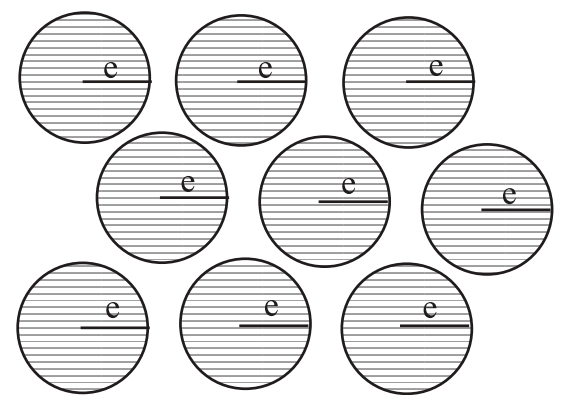
\includegraphics[scale=0.6]{../img/codewordsball.png}
\caption{Bola codeword yang tidak saling overlap}
\label{fig:codewordsball}
\end{figure}

Notasi umum kode biner adalah $(n,M,d)_2$. Kita bisa asumsikan ada $M$ bola yang tidak saling bersinggungan atau berpotongan, dengan radius bola $e$ seperti pada Gambar \ref{fig:codewordsball}. Jarak antara satu bola dengan bola yang lain adalah minimal $d$, sehingga didapatkan Persamaan \ref{eq:de}.
\begin{equation} \label{eq:de}
d = 2e + 1
\end{equation}

Sebuah kode biner $(n,M,d)_2$ dapat dibangkitkan dari kombinasi linear dari setiap baris pada generator matrix $[n,m,d]_2$ di mana $2^m = M$. Generator matriks $G$ adalah matriks berukuran $n \times m$, dapat juga disebut basis dari sebuah kode biner \cite{VanLint2016}. Contoh kode biner $(6,8,3)_2$ pada Gambar \ref{fig:binarycode683} dapat dibangkitkan dari generator matriks $[6,3,3]_2$ pada Gambar \ref{fig:generator633}. Asumsikan bahwa setiap baris dari $[6,3,3]_2$ adalah $g_1$, $g_2$, and $g_3$, lalu kode biner $(6,8,3)_2$ adalah semua kombinasi linear penjumlahan dari semua vektor dalam bentuk ${\lambda}_1 g_1 + {\lambda}_2 g_2 + {\lambda}_3 g_3$ di mana $\lambda_{i} \in \mathbb{F}_2^6$.

\begin{figure}
\centering
\begin{BVerbatim}
100110
010101
001011
\end{BVerbatim}
\caption{Generator matrix $[6,3,3]_2$}
\label{fig:generator633}
\end{figure}

Dari sebuah kode biner, kita dapat membuat kode biner yang baru dengan memodifikasi kode biner yang sudah ada \cite{Huffman}. Modifikasi yang dapat dilakukan adalah menambah dan mengurangi kode. Dari sebuah kode biner $(n,M,d)_2$, dapat dilakukan pemotongan pada kolom tertentu sehingga kode biner menjadi $(n-1,M,d^\prime)_2$ di mana $d^\prime=d$ atau $d^\prime=d-1$. Begitu pula dengan penambahan kode, dari sebuah kode biner $(n,M,d)_2$, dapat dilakukan penambahan kode sehingga kode biner menjadi $(n+1,M,d^\prime)_2$ di mana $d^\prime=d$ atau $d^\prime=d+1$.

\section{Kolerasi kode biner dengan permasalahan Ulam non interaktif}

Tujuan dari permasalahan ini adalah untuk menghasilkan $n$ query. Diberikan sebuah matriks $L$ berukuran $n \times M$ berisi $n$ query. Kumpulan query ini dinotasikan dengan $L = \{\vec{q_1},\vec{q_2},\ldots,\vec{q_n}\}$ di mana $\vec{q_i} = \{s_1,s_2,\ldots,s_M\}$. Himpunan nilai $s_j$ yang mungkin adalah $s_j \in \{0,1\}$.

Diberikan sebuah vektor $\vec{z} \in \{z_1,z_2,\ldots,z_n\}$ di mana $z_i \in \{0,1\}$ berisi jawaban dari seluruh query secara berurutan, $z_i$ adalah jawaban dari $\vec{q_i}$. Jika $z_i=0$ berarti jawaban query $q_i$ adalah 'tidak' sehingg seluruh $s_j$ pada $\vec{q_i}$ harus ditambah dengan 1 dan jika $z_i=1$ berarti jawaban dari query $\vec{q_i}$ adalah 'ya' sehingga seluruh $s_j$ pada $\vec{q_i}$ ditambah dengan 0 (diabaikan).

Matriks $L^\top$ berukuran $M \times n$ adalah hasil transpose dari matriks $L$. Asumsikan $L^\top$ juga dapat disebut sebagai kode biner $(n,M,d)_2$ di mana $n$ adalah jumlah query, $M$ adalah panjang $S_M$, dan $d$ adalah $2e+1$ di mana $e$ adalah jumlah maksimal bohong. Tambahkan seluruh baris $\vec{c_j}$ pada $L^\top$ dengan $\vec{z}$. Maka jawaban dari permainan Ulam non-interaktif adalah $x = j$ di mana $j$ adalah index dari baris $c$ pada $L^\top$ yang memiliki bobot $wt(\vec{c_j}) > n-e$.

\begin{lemma}
Diketahui integer $n$, $M$, dan $d$. Jika $L^\top$ adalah kode biner $(n,M,d)_2$ yang valid, maka jika setiap codeword $\vec{c}$ pada $L^\top$ ditambah dengan $\vec{z} \mid \vec{z} \in \mathbb{F}_2^n$ maka hasilnya akan tetap menjadi kode biner $(n,M,d)_2$ yang valid.
\end{lemma}

\begin{proof}
Jika $d_H(\vec{v_i},\vec{w_j}) \ge d \mid \vec{v_i},\vec{w_j} \in L^\top$ maka
\begin{align*}
d_H(\vec{v_i}+\vec{z},\vec{w_j}+\vec{z}) &\ge d \\
wt(\vec{v_i}+\vec{w_j}+\vec{z}+\vec{z}) &\ge d \\
wt(\vec{v_i}+\vec{w_j}) &\ge d \\
d_H(\vec{v_i},\vec{w_j}) &\ge d \\
\end{align*}
Jadi jika $d_H(\vec{v_i},\vec{w_j}) \ge d$ maka $d_H(\vec{v_i}+\vec{z},\vec{w_j}+\vec{z}) \ge d$.
\end{proof}

Penanya memenangkan permainan jika $L^\top$ memiliki paling banyak satu baris dengan $wt(\vec{c}) \ge n-e$. Jika hanya ada satu row, maka row tersebut adalah jawaban permainan. Jika tidak ada satu row pun yang memenuhi, penanya tetap memenangkan permainan karena penjawab melakukan kecurangan, melakukan bohong untuk semua angka lebih dari batas yang ditetapkan.

Untuk meyakinkan bahwa setelah seluruh jawaban $\vec{z}$ diberikan dan diaplikasikan ke matrix $L$ dan tidak pasti hanya ada 1 baris yang memiliki nilai $1$ antara $n-e \le wt(\vec{c_j}) \le n$, adalah dengan memastikan bahwa jarak Hamming setiap row yang berbeda pada $L^\top$ adalah minimal $d$.

\begin{lemma}
Diketahui integer $n$, $M$, dan $d$. Jika $L^\top$ adalah kode biner $(n,M,d)_2$ yang valid, maka pasti hanya ada paling banyak satu codeword $\vec{c}$ yang memiliki $0 \le wt(\vec{c}) \le e$.
\end{lemma}

\begin{proof}
Jika ada codeword $c$ di mana $0 \le wt(c) \le e$ maka $wt(\vec{v}) > e$ di mana $\vec{v} \neq c$. Pembuktian dapat dibuktikan dengan dua kasus.\\

1) Jika $wt(\vec{c}) = 0$ maka
\begin{align*}
d_H(\vec{c},\vec{v}) &\ge d \mid \vec{c} \neq \vec{v} , \vec{v} \in L^\top \\
wt(\vec{c} + \vec{v}) &\ge d \\
wt(\vec{v}) &\ge d \label{eq:proofd} \stepcounter{equation} \tag{\theequation}
\end{align*}
Sebelumnya telah disebutkan hubungan $d$ dan $e$ pada Persamaan \ref{eq:de}. Persamaan tersebut dapat diturunkan menjadi
\begin{equation} \label{eq:dge}
d > e
\end{equation}
Dengan memasukkan Persamaan \ref{eq:dge} ke Persamaan \ref{eq:proofd}, maka didapatkan
\begin{equation*}
wt(\vec{v}) > e
\end{equation*}

2) Jika $wt(\vec{c}) = e$ maka
\begin{align*}
d_H(\vec{c},\vec{v}) &\ge d \mid \vec{c} \neq \vec{v} , \vec{v} \in L^\top \\
wt(\vec{c}+\vec{v}) &\ge d \\
wt(\vec{c}) + wt(\vec{v}) \ge wt(\vec{c}+\vec{v}) &\ge d \\
wt(\vec{c}) + wt(\vec{v}) &\ge d \\
e + wt(\vec{v}) &\ge d \\
\intertext{Masukkan Persamaan \ref{eq:de} untuk mensubstitusi $d$}\\
wt(\vec{v}) &\ge 2e+1-e \\
&\ge e+1\\
wt(\vec{v}) &> e
\end{align*}
Jadi jika ada codeword $c$ di mana $0 \le wt(c) \le e$ maka $wt(\vec{v}) > e$ di mana $\vec{v} \neq c$.
\end{proof}

Dari pembuktian diatas, dapat disimpulkan bahwa untuk menyelesaikan permainan pencarian Ulam non-interaktif dengan batas pencarian $M$ dan maksimal kebohongan $e$, transpose dari $n$ query yang dibuat harus membentuk kode biner $(n,M,d)_2$.
